% Created 2022-07-12 Tue 19:12
% Intended LaTeX compiler: pdflatex
\documentclass[presentation,aspectratio=1610]{beamer}
\usepackage[utf8]{inputenc}
\usepackage[T1]{fontenc}
\usepackage{graphicx}
\usepackage{grffile}
\usepackage{longtable}
\usepackage{wrapfig}
\usepackage{rotating}
\usepackage[normalem]{ulem}
\usepackage{amsmath}
\usepackage{textcomp}
\usepackage{amssymb}
\usepackage{capt-of}
\usepackage{hyperref}
\usepackage{khpreamble}
\usepackage{amssymb}
\DeclareMathOperator{\shift}{q}
\DeclareMathOperator{\diff}{p}
\usetheme{default}
\author{Kjartan Halvorsen}
\date{2021-07-12}
\title{Digital PID}
\hypersetup{
 pdfauthor={Kjartan Halvorsen},
 pdftitle={Digital PID},
 pdfkeywords={},
 pdfsubject={},
 pdfcreator={Emacs 26.3 (Org mode 9.4.6)}, 
 pdflang={English}}
\begin{document}

\maketitle


\section{Discretization - repetición}
\label{sec:org2a507e9}
\begin{frame}[label={sec:org7dfdbb8}]{Mapping of the stable region of the s-plane when discretizing the controller}
\pause

\begin{center}
 \includegraphics[width=0.7\linewidth]{../../figures/mapping-stable-s-region.png}\\
\end{center}

\pause

\alert{Activity} Which of the above mappings of the left-half plane of the s-plane corresponds to A) the bilinear transformation (Tustin's approximation), B) the forward difference approximation, C) the backward difference approximation?
\end{frame}

\begin{frame}[label={sec:orgb3452e6}]{Mapping of the stable region of the s-plane}
\begin{center}
 \includegraphics[width=0.79\linewidth]{../../figures/fig8-2.png}\\
{\tiny Åström and Wittenmark \emph{Computer-controlled systems}}
\end{center}
\end{frame}


\section{PID}
\label{sec:org3fee3aa}
\begin{frame}[label={sec:orgddb36f2}]{ISA form of the PID}
ISA - International Society of Automation

\[ F(s) = K_c\left( 1 + \frac{1}{T_i s} + T_d s\right) \]

With low-pass filter for the derivative part

\[ F(s) = K_c\left( 1 + \frac{1}{T_i s} + \frac{T_d s}{\frac{T_d}{N} s + 1}\right), \quad N \approx 3\; - \; 10 \]
\end{frame}

\begin{frame}[label={sec:orgc54bb43}]{PID with derivative action only on the process variable}
\begin{center}
  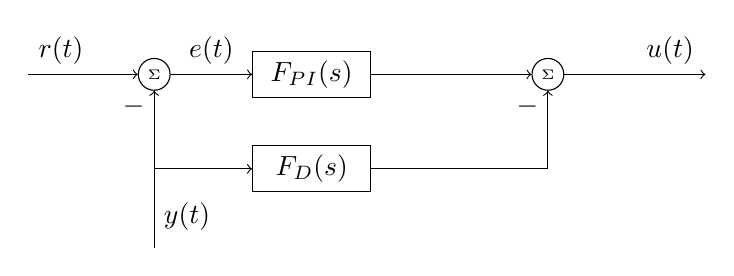
\begin{tikzpicture}[node distance=22mm, block/.style={rectangle, draw, minimum width=15mm}, sumnode/.style={circle, draw, inner sep=2pt}]

    \node[coordinate] (input) {};
    \node[sumnode, right of=input, node distance=16mm] (sum) {\tiny $\Sigma$};
    \node[block, right of=sum, node distance=20mm] (pi)  {$F_{PI}(s)$};
    \node[block, below of=pi, node distance=12mm] (dd)  {$F_{D}(s)$};
    \node[sumnode, right of=pi, node distance=30mm] (sum2) {\tiny $\Sigma$};
    \node[coordinate, below of=sum, node distance=22mm] (yy) {};
    \node[coordinate, right of=sum2, node distance=20mm] (output) {};

    \draw[->] (input) -- node[above, pos=0.3] {$r(t)$} (sum);
    \draw[->] (sum) -- node[above] {$e(t)$} (pi);
    \draw[->] (sum2) -- node[above, near end] {$u(t)$} (output);
    \draw[->] (yy) -- node[right, pos=0.2] {$y(t)$} node[pos=0.9, left] {$-$} (sum);
    \draw[->] (pi) -- node[above, near end] {} (sum2);
    \draw[->] (dd) -| node[left, pos=0.9] {$-$} (sum2);
    \draw[->] (yy) |- (dd);

  \end{tikzpicture}
\end{center}

\[ U(s) = \underbrace{K_c\left( 1 + \frac{1}{T_i s} \right)}_{F_{PI}(s)} E(s) - \underbrace{K_c\frac{T_d s}{\frac{T_d}{N} s + 1}}_{F_{D}}Y(s)\]
\end{frame}

\section{Discretización del PID}
\label{sec:orgc14bf56}
\begin{frame}[label={sec:orgb59510c}]{Common discretization of the PID}
\begin{center}
  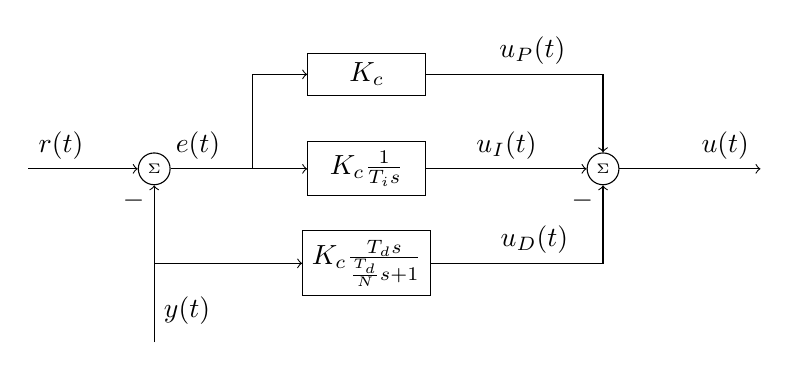
\begin{tikzpicture}[node distance=22mm, block/.style={rectangle, draw, minimum width=15mm}, sumnode/.style={circle, draw, inner sep=2pt}]

    \node[coordinate] (input) {};
    \node[sumnode, right of=input, node distance=16mm] (sum) {\tiny $\Sigma$};
    \node[block, right of=sum, node distance=27mm] (pi)  {$K_c\frac{1}{T_is}$};
    \node[block, below of=pi, node distance=12mm] (dd)  {$K_c\frac{T_d s}{\frac{T_d}{N} s + 1}$};
    \node[block, above of=pi, node distance=12mm] (pp)  {$K_c$};
    \node[sumnode, right of=pi, node distance=30mm] (sum2) {\tiny $\Sigma$};
    \node[coordinate, below of=sum, node distance=22mm] (yy) {};
    \node[coordinate, right of=sum2, node distance=20mm] (output) {};

    \draw[->] (input) -- node[above, pos=0.3] {$r(t)$} (sum);
    \draw[->] (sum) -- node[above, pos=0.2] {$e(t)$} node[coordinate, pos=0.6] (copy) {} (pi);
    \draw[->] (sum2) -- node[above, near end] {$u(t)$} (output);
    \draw[->] (yy) -- node[right, pos=0.2] {$y(t)$} node[pos=0.9, left] {$-$} (sum);
    \draw[->] (pi) -- node[above, ] {$u_I(t)$} (sum2);
    \draw[->] (dd) -| node[left, pos=0.9] {$-$} node[above, pos=0.3] {$u_D(t)$} (sum2);
    \draw[->] (yy) |- (dd);
    \draw[->] (pp) -| node[above, pos=0.3] {$u_P(t)$} (sum2);
    \draw[->] (copy) |- (pp);


  \end{tikzpicture}
\end{center}

\[ U(s) = U_P(s) + U_I(s) - U_D(s) = K_cE(s) + K_c\frac{1}{T_i s} E(s) - K_c\frac{T_d s}{\frac{T_d}{N} s + 1}Y(s) \]

\alert{Activity} 1) Use the forward difference \(s \approx \frac{z-1}{h}\) for the integral part, and the backward difference \(s \approx \frac{z-1}{zh}\) for the derivative part. 2) Apply the inverse z-transform to obtain the controller in the form of a difference equation.
\end{frame}

\begin{frame}[label={sec:orgc818e6c}]{Common discretization of the PID  - Solution}
\begin{block}{Proportional part}
Very simple: \(u_P(kh) = K_c e(kh)\)
\end{block}
\begin{block}{Integral part}
Substitute \(s = \frac{z-1}{h}\) in the transfer function \(F_I(s) = \frac{K_c}{T_i} \frac{1}{s}\)
\[ F_{I,d}(z) = \frac{K_c}{T_i}\frac{1}{\frac{z-1}{h}} = \frac{K_c}{T_i} \frac{h}{z-1}\]
\[U_I(z) = \frac{K_c}{T_i} \frac{h}{z-1} E(z), \qquad \text{}\]
\[U_I(z)(z-1) = \frac{K_c}{T_i} h E(z), \qquad \text{Apply inverse z-transform}\]
\[ u_I(kh+h) - u_I(kh) = \frac{K_c}{T_i} h e(kh) \qquad \Leftrightarrow \qquad u_I(kh+h) = u_I(kh) + \frac{K_c}{T_i} h e(kh)\]
\end{block}
\end{frame}

\begin{frame}[label={sec:orgb0f28b9}]{Common discretization of the PID  - Solution}
\begin{block}{Derivative part}
Substitute \(s = \frac{z-1}{zh}\) in the transfer function \(F_D(s) = K_c \frac{T_d s}{\frac{T_d}{N} s + 1}\)
\[ F_{D,d}(z) = K_c\frac{T_d \frac{z-1}{zh}}{\frac{T_d}{N}\cdot\frac{z-1}{zh}+1} 
         = K_c \frac{T_d(z-1)}{\frac{T_d}{N}(z-1) + zh} 
= K_c \frac{T_d(z-1)}{(\frac{T_d}{N}+h)z -\frac{T_d}{N}} \]
\[ U_D(z) = K_c \frac{T_d(z-1)}{(\frac{T_d}{N}+h)z -\frac{T_d}{N}} Y(z)\]
\[ \Big((\frac{T_d}{N}+h)z -\frac{T_d}{N}\Big) U_D(z) = K_cT_d(z-1) Y(z), \qquad \text{Apply the inverse z-transform} \]
\[ (\frac{T_d}{N}+h)u_D(kh+h) -\frac{T_d}{N}u_D(kh) = K_cT_d\big(y(kh+h) - y(kh)\big)\]
\end{block}
\end{frame}

\begin{frame}[label={sec:orgffa2860}]{The discrete PID algorithm}
\small

\begin{align*}
&\text{Calculated:}  \;  \alpha_1 = \frac{\frac{T_d}{N}}{\frac{T_d}{N} + h},\; \alpha_2 = K_c\frac{T_d}{\frac{T_d}{N} + h}, \; \beta = K_c \frac{h}{T_i}\\
&\text{Stored:}  \;  y(kh-h), \; u_I(kh-h), \; u_D(kh-h)\\
& \text{\textcolor{green!60!black}{Sample signals:}} \; r(kh), \; y(kh)\\
&e(kh) = r(kh) - y(kh)\\
&u_P(kh) = K_ce(kh)\\
&u_D(kh) = \alpha_1 u_D(kh-h) + \alpha_2\big(y(kh) - y(kh-h)\big)\\
&u(kh) = u_P(kh) + u_I(kh-h) - u_D(kh), \qquad \text{\textcolor{red}{Send to DAC}}\\
&u_I(kh) = u_I(kh-h) + \beta e(kh)
\end{align*}

\begin{center}
  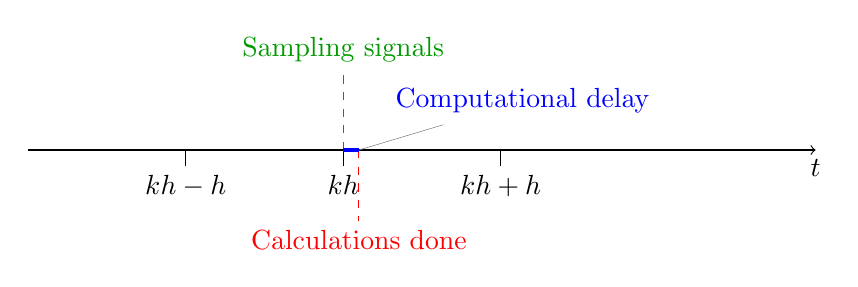
\begin{tikzpicture}
    \draw[->] (0,0) -- (10,0) node[below] {$t$};
    \draw (2,0) -- (2,-0.2) node[below] {$kh-h$};
    \draw (4,0) -- (4,-0.2) node[below] {$kh$};
    \draw (6,0) -- (6,-0.2) node[below] {$kh+h$};
    \draw[green!60!black, dashed] (4,0) -- (4, 1) node[above] {Sampling signals};
    \draw[red, dashed] (4.2,0) -- (4.2, -0.9) node[below] {Calculations done};
    \draw[blue, ultra thick] (4,0) -- (4.2,0) node[coordinate, pin=45:{Computational delay}] {};
  \end{tikzpicture}
\end{center}
\end{frame}
\end{document}